\renewcommand{\rmdefault}{ptm} % Arial:phv, Roman:ptm
\renewcommand{\sfdefault}{ptm} % Arial
\documentclass[journal]{IEEEtran} % onecolumn,12pt
\hyphenation{op-tical net-works semi-conduc-tor}

%\usepackage{program}
\usepackage[caption=false,font=footnotesize]{subfig}
\usepackage{color}
\usepackage{cite}
\usepackage{amsmath}
\usepackage{amssymb}
\usepackage{amsthm}
\usepackage{graphicx}
\newtheorem{theorem}{Theorem}
\newtheorem{prop}{Proposition}
\newcommand{\indep}{\rotatebox[origin=c]{90}{$\models$}}
\usepackage{epstopdf}
\usepackage{comment}
\usepackage{multirow}
\usepackage{algorithm2e}
\usepackage{threeparttable}
\usepackage{booktabs}
\usepackage{multirow}
\usepackage{amsmath}
\graphicspath{{./Pictures/}}
\definecolor{orange}{rgb}{1,0.5,0}


\begin{document}
\title{The Bidding Strategy for Load Service Entity in Real-Time Virtual Retail Market using Stochastic Dual Dynamic Probability}

\author{Wonseok~Choi,~\IEEEmembership{Student Member,~IEEE,} 
	~Duehee~Lee,~\IEEEmembership{Member,~IEEE,}
	}


% The paper headers
\markboth{IEEE Transaction on Smart Grid}%
{Shell \MakeLowercase{\textit{et al.}}: Bare Demo of IEEEtran.cls for Journals}
\maketitle

\begin{abstract}
As the will of decarbonization is realized in the electricity market around the world, the renewable energy sources are penetrating in the system. However, the system stability tend s to become unstable due to reduction of generation from underlying source and intermittent characteristics of renewable energy. Therefore, it is difficult to secure system stability only by controlling generation, so the system is trying to induce consumer participation in the market. Consumer participation in the market is achieved by controlling demand, to do this, the price signal of load service entities (LSE) is required. The real-time pricing (RTP) is one of the tariff that can induce demand shifting by changing retail prices in real time. In this paper, we propose bidding strategy of LSE for RTP tariff. The proposed bidding strategy has a objective function which maximizes income of LSE and uses stochastic dual dynamic programming (SDDP) theory to consider probabilities and time elements. In addition, after establishing proposed theory, we show example of use of bidding strategy through numerical experiment.
\end{abstract}



%================================================================



\section{Introduction}
%%%%%%%%%%%%%======== Notation =======%%%%%%%%%%%%%
%%%%%%%%%%%%%======== Why we need RTP tariff =======%%%%%%%%%%%%%

%%%%%%%%%%%%%-------- Decarbonization --------%%%%%%%%%%%%%
\IEEEPARstart{A}{ll} over the world, the awareness of global warming is increasing, and the will to decarbonize is spreading rapidly~\cite{rockstrom2017roadmap}. As a result, renewable energy resource was discussed as a solution for above problem~\cite{shahzad2012need} and is penetrating the electricity system~\cite{Bull2001,ranalder2021renewables}. 

%%%%%%%%%%%%%-------- Renewable energy problem --------%%%%%%%%%%%%%
However, renewable energy resources do not have a positive effect on the system.  Solar and wind power energy, which are the main renewable resource, output power depend on natural force rather than producer's control. Thus, due to these intermittent characteristic, renewable energy contains uncertainty in power supply, which cause less system reliability~\cite{zahedi2011review}. Also, the power supply reliability problem extends to problems such as voltage drop, frequency drop, and system inertia, ramping issue, and as a result, a high penetration of renewable energy become a motive to lower system stability\cite{santoso2012electrical, dreidy2017inertia, wang2016enhancing}.

%%%%%%%%%%%%%-------- Problem another enetity --------%%%%%%%%%%%%%
To solve above system instability problem caused by the renewable energy penetration, each entities interested in electricity system show various effort. In Genco case, many power generation forecasting methodology have been introduced~\cite{lee2013short, lee2016probabilistic, agoua2017short}. Generator can participate in dispatch market using these forecasted values and meet a target capacity through fine-tuning using energy storage system (ESS)~\cite{shim2013synergistic}. Also, system operators establish operation planning considering stochastic factors and enhance flexibility by introducing energy management system (EMS) for power distribution networks~\cite{palma2013microgrid}.

%%%%%%%%%%%%%-------- Problem in LSE --------%%%%%%%%%%%%%
Grid instability also affects load serving entities (LSE). Due to intermittent characteristics of renewable energy, general energy balance cannot be achieved day-ahead market, which means that the price signal determined as day-ahead market may be different from the actual electricity price in target day. Most LSEs adopt flat-rate tariffs which has constant cost regardless of time. However, LSE's flat-rate charges are set amount that can fully recover costs incurred in the wholesale market, and as system volatility increases, the full recovery at a flat-rate become unstable.

%%%%%%%%%%%%%-------- Dynamic tariffs --------%%%%%%%%%%%%%
Thus, many LSEs are attempting to introduce dynamic pricing (DP). DP is classified into various retail tariffs according to price volatility. Examples of DP, time of use (TOU) that has several fixed rates depending on the time or seoson, critical peak pricing (CPP) that change rates in the peak load period. In addition, there is real time pricing (RTP), which means a tariff that changes retail rates in real time. Below Fig~\ref{type_DP} shows the premium ratio within tariffs according to price volatility.

\begin{figure}[t!]
\centering
  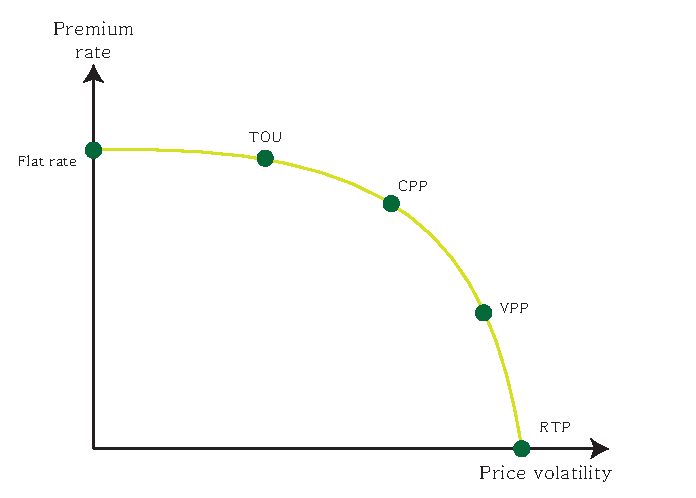
\includegraphics[width=3.5in]{type_DP}
\caption{The type of dynamic pricing}
\label{type_DP}       % Give a unique label
\end{figure}

%%%%%%%%%%%%%-------- RTP advantage --------%%%%%%%%%%%%%
RTP has several advantages, first of all, there is no or minimum rate of \textit{premium} in the tariff. The \textit{premium} is an additional fee for LSE to avoid risk of price volatility, it has higher \textit{premium} cost when use non-dynamic pricing. Therefore, RTP can supply electricity cheaper than general tariffs~\cite{boeve2021asset}. Second, RTP expands the demand response (DR). Adopting the RTP tariff, it provides current electricity prices tot consumers in real time, which in itself becomes a price signal and can induce efficient demand shifting. Considering the advantages of RTP and the acceleration of system volatility, RTP adoption rate will be increased.

%%%%%%%%%%%%%-------- Importance of RTP Bidding strategy --------%%%%%%%%%%%%%
Considering prospect of RTP, many literatures describe operating strategies of each entity in power system. In~\cite{roozbehani2012volatility, samadi2011optimal} deals with energy balancing issue based on price signal of RTP, and~\cite{pei2016optimal, wang2020day} describe the aggregators' operating strategy when considering the demand shifting in DR market. In particular, LSEs are institution that directly operates RTP, and there are several literature aimed at maximizing LSE's revenue~\cite{kazemi2014risk, safdarian2013impacts, alipour2018hedging, samadi2010optimal}.

%%%%%%%%%%%%%-------- The problem of existing literatures --------%%%%%%%%%%%%%
\textcolor{red}{However, the papers related to operation LSE strategy have some limitations. In~\cite{kazemi2014risk, safdarian2013impacts} basically a bidding strategy for variance demand was established by interpreting demand elasticity as sensitivity to price. But, citing the results represented in~\cite{boeve2021asset, fabra2021estimating}, simple bidding strategies according to price variance in RTP tariff is only strategy to guarantee risk of revenue from price signal, but does not role controlling demand. In addition to along with~\cite{kazemi2014risk},~\cite{wang2020day, alipour2018hedging} have the results represented by a confidence interval come from a scenario. However, these results are in form of transferring stochastic part of strategy to methodological users, resulting that users need another optimization.}

%%%%%%%%%%%%%-------- The problem of existing literatures --------%%%%%%%%%%%%%
In this paper, we purpose a improved LSEs bidding strategy considering the previous problems and the features are as follow: 

First of all, the purpose is to determine the optimal bidding capacity using the stochastic dual dynamic programming (SDDP) theory. SDDP is a theory that can be applied when entire scope is divided into some stages and each stage has probabilistic characteristics. Generally, stages are specified by time, electric vehicle (EV) charging mapping~\cite{fallah2020charge} or unit commitment (UC) uses this methodology in power system~\cite{zou2018multistage, hreinsson2019continuous}. Using the SDDP theory, we can consider factor about uncertainty in each stage, and address optimal of current stage in process of moving on next stage.

\textcolor{red}{Second, using exponential probability distribution, estimate the elasticity of demand. SDDP requires independent probabilistic factor for each stage. Therefore, in this paper, demand sensitivity to price, that is, demand elasticity is set as probabilistic factor. In addition, general demand elasticity has a right-hand curve for prices, so exponential distribution that can be reflected and approximated is used.}

Third, we create reference demand and focus on demand variance rather than absolute demand. By setting variance as variable of optimization, probability factor using in bidding process can be intuitively interpreted, and results according to each stage can be reviewed through numerical analysis.


%%%%%%%%%%%%%-------- Contribution --------%%%%%%%%%%%%%
\textcolor{red}{The by-products of this paper is demand curve for prices using probability distribution and bidding strategy methodology using SDDP. Using demand curve, it is possible to induce expansion of DR market in short term and establish long-term system operation planning that includes demand shifting. In addition, the improved bidding strategy can minimize risk of operation through stochastic analysis in volatile market, and plan new direction because chain analysis through artificial price control is possible. Eventually, when price risk for LSEs is completely resolved, there is no need to share with consumers, which cause price cuts.}

\section{Market}

\section{Theory Description}
\subsection{SDDP}

\section{Bidding Strategy Methodology}
\newpage








\section{Conclusion}


















\ifCLASSOPTIONcaptionsoff
  \newpage
\fi


\bibliographystyle{IEEEtran}
\bibliography{sddp_1}



\end{document}







